\renewcommand{\theequation}{\theenumi}
\renewcommand{\thefigure}{\theenumi}
\renewcommand{\thetable}{\theenumi}
\begin{enumerate}[label=\thesection.\arabic*.,ref=\thesection.\theenumi]
\numberwithin{equation}{enumi}
\numberwithin{figure}{enumi}
\numberwithin{table}{enumi}

\item Two independent random variables \(X\) and \(Y\)
are uniformly distributed in the interval [-1,1].The probability that max \{\(X\),\(Y\)\} is less than \(\frac{1}{2}\) is
\begin{enumerate}[label={\Alph*)}]
    \item 3/4
    \item 9/16
    \item 1/4
    \item 2/3
\end{enumerate}
\solution
\begin{lemma}
    CDF of the random variable X is : 
    \begin{equation}
       F_X\brak{x}=
       \begin{cases}
       0 & x\leq-1\\
       \frac{1}{2}(x+1) & -1<x<1\\
       1 & x\geq1 
       \end{cases}\label{indep/1/2.0.1}
    \end{equation}
   \end{lemma}
   \begin{proof}
   Given \(X\) is uniformly distributed in [-1,1] i.e. \(X\) \(\sim\) U(-1,1)
   \\PDF of \(X\) : 
   \begin{equation}
       f_{X}\brak{x}=
       \begin{cases}
        0 & x\leq-1\\
        \frac{1}{2} & -1\leq x\leq 1\\
        0 & x\geq1
       \end{cases}
   \end{equation}
   For  \(-1\leq x\leq 1\)
   \begin{align}
     F_{X}\brak{x}&=\Pr\brak{X\leq x}\\
     &=\int_{-1}^x\frac{1}{2}dx\\
     &=\frac{1}{2}(x+1)
   \end{align}
   Hence \eqref{indep/1/2.0.1} is proved
   \end{proof}
   \begin{lemma}
    CDF of the random variable Y is : 
    \begin{equation}
       F_X\brak{x}=
       \begin{cases}
       0 & x\leq-1\\
       \frac{1}{2}\brak{x+1} & -1<x<1\\
       1 & x\geq1 
       \end{cases}\label{indep/1/2.0.5}
    \end{equation}
   \end{lemma}
   \begin{proof}
   Given \(Y\) is uniformly distributed in [-1,1] i.e. \(Y\)\(\sim\) U(-1,1)
   \\PDF of \(Y\) : 
   \begin{equation}
       f_{Y}\brak{y}=
       \begin{cases}
        0 & y\leq-1\\
        \frac{1}{2} & -1\leq y\leq 1\\
        0 & y\geq1
       \end{cases}
   \end{equation}
   For  \(-1\leq y\leq 1\)
   \begin{align}
     F_{Y}\brak{y}&=P(Y\leq y)\\
     &=\int_{-1}^y\frac{1}{2}dy\\
     &=\frac{1}{2}\brak{y+1}
   \end{align}
   Hence \eqref{indep/1/2.0.5} is proved
   \end{proof}
   \begin{lemma}
   \begin{align}
       \Pr\brak{{max\{X,Y\}<\frac{1}{2}}} = \frac{9}{16}\label{indep/1/2.0.11}
   \end{align}
   \end{lemma}
   \begin{proof}
   \({max\{X,Y\}}<\frac{1}{2} \implies\) \(X<\frac{1}{2}\) , \(Y<\frac{1}{2}\)\\
   Given \(X\) and \(Y\) are independent,
   \begin{align}
       Pr(X<\frac{1}{2},&Y<\frac{1}{2})\\
       &=\Pr\brak{X <\frac{1}{2}}\times \Pr\brak{Y <\frac{1}{2}}\\
       &=F_X\brak{\frac{1}{2}} \times F_Y\brak{\frac{1}{2}}\\
      &=\frac{3}{2}\times\frac{1}{2}\times\frac{3}{2}\times\frac{1}{2}\\
       &=\frac{9}{16}
   \end{align}
   Hence \eqref{indep/1/2.0.11} is proved
   \end{proof}
   Option B is correct

\item Three fair cubical dice are thrown simultaneously. The probability that all three dice have the same number of dots on the faces showing up is (up to third decimal place)...........
\solution
Let 
\begin{align}
X_{1},X_{2},X_{3} \in \{1,2,3,4,5,6\}
\end{align}
represent the three dice.

Since, all the three are fair dice, the probability of any dice showing a particular number is given by
\begin{align}
 \pr{X=i} =
    \begin{cases}
      \frac{1}{6} & \text{i=1,2,3,4,5,6}\\
       0 & \text{otherwise}
    \end{cases}       
\end{align}
If all the dice show a particular number i,
\begin{align}
\implies \pr{X_{1} =X_{2}=X_{3}=i}
\end{align}
Since the events are independent, 
\begin{multline}\label{eq1}
  \pr{X_{1} =X_{2}=X_{3}=i}\\
  =  \pr{X_{1}=i}\pr{X_{2}=i}\pr{X_{3}=i}
\end{multline}
where i=1,2,3,4,5,6.\\
There are 6 faces on a cubical dice. Hence, there are six cases in which all the dice show the same number
\begin{align}
 \pr{X_1 =X_2 =X_3}&=\sum^{6}_{i=1} \pr{X_{1} =X_{2}=X_{3}=i}
 \end{align}
 From \eqref{eq1},we have
 \begin{multline}
\pr{X_1 =X_2 =X_3}
\\=\sum^{6}_{i=1}\pr{X_{1}=i}\pr{X_{2}=i}\pr{X_{3}=i}
\end{multline}
\begin{align}
 &=\sum^{6}_{i=1}\brak{\frac{1}{6}}\brak{\frac{1}{6}}\brak{\frac{1}{6}}\\
 &=\frac{1}{36}
\end{align}
%
\item Given Set A = [2,3,4,5] and Set B = [11,12,13,14,15], two numbers are randomly selected,one from each set. What is probability that the sum of the two numbers equals 16?

\begin{enumerate}
\begin{multicols}{4}
\setlength\itemsep{2em}

\item $
0.20
$
\item $
0.25
$
\item $
0.30
$
\item $
0.33
$

\end{multicols}
\end{enumerate}
\solution
Given,\\
Set A= [2,3,4,5]\\
Set B= [11,12,13,14,15]\\

Total number of element in the sample space is 20.\\

Let us define a random variable$ X \in \cbrak{0,1}$\\
\begin{table}[ht]
    \centering
    \begin{tabular}{|c|c|}
    \hline
    X=0 & the event when A+B=16\\
    \hline
    X=1 & the event when A+B $\neq$ 16\\
    \hline
    \end{tabular}
    \caption{Random Variables}
    \label{tab:Random Variables}
\end{table}

Now, probability of selecting an element from set A such that \pr{X=0} is
\begin{equation}
   \tag{7.1}
    \pr{X=0}=\pr{A+B=16}=1
\end{equation}

So,the probability of selecting an element from set B after selecting an element from set A such that \pr{X=0} is
\begin{equation}
    \tag{7.2}
    \pr{X=0}=\pr{A+B=16}= \frac{1}{5}
\end{equation}

Therefore,\\
Overall probability of randomly choosing elements from set A and set B such that \pr{X=0}is
\begin{align}
    \tag{7.3}
    \pr{X=0}&=\pr{A+B=16}\\
    \tag{7.4}
    \pr{X=0}&=1 \times \frac{1}{5}\\
    \tag{7.5}
    \pr{X=0}&= \frac{1}{5}=0.2
\end{align}


\begin{table}[ht]
    \centering
    \begin{tabular}{|c|c|c|}
    \hline
    X & 0 & 1\\
    \hline
    $\pr{X}$ & $\frac{1}{5}$ & $\frac{4}{5}$\\
    \hline
    \end{tabular}
    \caption{Probability distribution table}
    \label{tab:Probability distribution table}
\end{table}

Therefore, the correct option is (a).
%
\item Two independent random variables X and Y are uniformly distributed in the interval $[-1,1]$.The probability that max$[X,Y]$ is less than $\dfrac{1}{2}$ is

\begin{enumerate}
\begin{multicols}{4}
\setlength\itemsep{2em}

\item $
\dfrac{3}{4}
$
\item $
\dfrac{9}{16}
$
\item $
\dfrac{1}{4}
$
\item $
\dfrac{2}{3}
$
\end{multicols}
\end{enumerate}
%
\item A fair dice is tossed two times. The probability that the second toss result in a value that is higher than the first toss is
\begin{enumerate}
\begin{multicols}{4}
\setlength\itemsep{2em}
\item $
\dfrac{2}{36}
$
\item $
\dfrac{2}{6}
$
\item $
\dfrac{5}{12}
$
\item $
\dfrac{1}{2}
$
\end{multicols}
\end{enumerate}
%
\solution
Given, a fair die, which is tossed twice. Let the random variable $X_{i}\in\{1,2,3,4,5,6\},i=1,2,$ represent the outcome of the number on the die in the first, second toss respectively.  
The probability  mass function (PMF) for a fair die is expressed as \begin{align}
    \tag{26.1}
    \label{eq:pmf}
    p_{X_{i}}(n)=\Pr(X_{i}=n) = 
	\begin{cases}
	\dfrac{1}{6}, & 1\leq n\leq6 \\~\\[-1em]
	0, & otherwise
	\end{cases}
\end{align}
Using \eqref{eq:pmf}, the cumulative distribution function (CDF) is obtained to be
\begin{align}
    \tag{26.2}
    F_{X_{i}}(r)=\Pr(X_{i}\leq r) = 
	\begin{cases}
	\dfrac{r}{6}, & 1\leq r\leq6 \\~\\[-1em]
	1, & r \geq 7 \\~\\[-1em]
	0, & otherwise
	\end{cases}
	\label{eq:26.2}
\end{align}
\begin{align}
    \tag{26.3}
    X_{1}<X_{2}\Rightarrow X_{2}=k,X_{1}\leq k-1
\end{align}
$\because X_{1},X_{2}$ are independent,
\begin{align}
    \tag{26.4}
    Pr(X_{1}<X_{2})=E\left[F_{X_{1}}(X_{2}-1)\right]
    \label{eq:probeqn}
\end{align}
After unconditioning \eqref{eq:probeqn}, we get
\begin{align}
    \tag{26.5}
    Pr(X_{1}<X_{2})=\sum_{k=1}^{6}p_{X_{2}}(k) F_{X_{1}}(k-1)
\end{align}
Substituting \eqref{eq:pmf} and \eqref{eq:26.2}, we get
\begin{align}
    \tag{26.6}
    Pr(X_{1}<X_{2})=\sum_{k=1}^{6}\dfrac{1}{6}\left(\dfrac{k-1}{6} \right)
\end{align}
On solving, we get
\begin{align}
    \tag{26.7}
    Pr(X_{1}<X_{2})=\dfrac{5}{12}\text{(option (C))}
\end{align}
\begin{table}[h!]
\centering
\caption{Cases and their theoretical probabilities}
\label{table:1}
\begin{tabular}{|c||c|c|c|}
    \hline
    Case & $X_{1}<X_{2}$& $X_{1}>X_{2}$& $X_{1}=X_{2}$ \\
    \hline
    %& & &\\
    Probability & $\dfrac{5}{12}$ & $\dfrac{5}{12}$ & $\dfrac{1}{6}$\\[1ex]
    \hline
\end{tabular}
\end{table}
%
\item Consider two independent random variables X and Y with identical distributions. The variables X and Y take value 0, 1 and 2 with probabilities $\dfrac{1}{2}$, $\dfrac{1}{4}$ and $\dfrac{1}{4}$ rrespectively. What is the conditional probability $P(X+Y = 2|X-Y =0)$?

\begin{enumerate}
\begin{multicols}{4}
\setlength\itemsep{2em}

\item 0
\item $\dfrac{1}{16}$
\item $\dfrac{1}{6}$
\item 1

\end{multicols}
\end{enumerate}
%
\solution
The values that the random variable X can take along with its probabilities are given by
\begin{table}[h]
\centering
\begin{tabular}{|l|l|l|l|}
\hline
X             & 0             & 1             & 2             \\ \hline
$\Pr\brak{X}$ & $\frac{1}{2}$ & $\frac{1}{4}$ & $\frac{1}{4}$ \\ \hline
\end{tabular}
\end{table}
\newline
The values that the random variable Y can take along with its probabilities are given by
\begin{table}[h]
\centering
\begin{tabular}{|l|l|l|l|}
\hline
Y             & 0             & 1             & 2             \\ \hline
$\Pr\brak{Y}$ & $\frac{1}{2}$ & $\frac{1}{4}$ & $\frac{1}{4}$ \\ \hline
\end{tabular}
\end{table}
\begin{align}
\Pr\brak{X-Y=0}=\frac{1}{2}\times\frac{1}{2}+\frac{1}{4}\times\frac{1}{4}+\frac{1}{4}\times\frac{1}{4}=\frac{6}{16}\\
\Pr\brak{(X+Y=2),(X-Y=0)}=\frac{1}{4}\times\frac{1}{4}=\frac{1}{16}
\end{align}
\begin{align}
\Pr\brak{X+Y=2\:|\:X-Y=0}\notag\\
=&\frac{\Pr\brak{(X+Y=2),(X-Y=0)}}{\Pr\brak{X-Y=0}}\notag\\
=&\frac{\frac{1}{16}}{\frac{6}{16}}=\frac{1}{6}
\end{align}
%
\item Let X and Y be two statistically independent random variables uniformly distributed in the range $(-1,1)$ and $(-2,1)$ respectively. Let $Z = X+Y$, then the probability that $[Z\leqslant-2]$ is
\begin{enumerate}
\begin{multicols}{4}
\setlength\itemsep{2em}
\item zero
\item $\dfrac{1}{6}$
\item $\dfrac{1}{3}$
\item $\dfrac{1}{12}$
\end{multicols}
\end{enumerate}
%
\solution
\section{Answer}
Option (D) $\dfrac{1}{12}$
\section{Solution}
X and Y are two independent random variables. \\
Let
\begin{align}
    p_X\brak{x} &= \Pr\brak{X=x} \\
    p_Y\brak{y} &= \Pr\brak{Y=y}  \\
    p_Z\brak{z} &= \Pr\brak{Z=z}
\end{align}
be the probability densities of random variables X ,Y and Z. \\
X lies in range(-1,1), therefore,
\begin{align}
    \int_{-1}^{1} p_X\brak{x} \,dx  &=1 \\
    2 \times p_X\brak{x}  &= 1 \\
     p_X\brak{x} =1 /2
\end{align}
Similarly for Y we have,
\begin{align}
    \int_{-2}^{1} p_Y\brak{y} \,dy  &=1 \\
    3 \times p_Y\brak{y}  &= 1  \\
     p_Y\brak{y} =1 /3
\end{align}
The density for X is \\
\begin{align}
\label{eq:_pdf_x}
p_{X}(x)  = 
\begin{cases}
\frac{1}{2} & -1 \le x \le 1
\\
0 & otherwise
\end{cases}
\end{align}
We have ,
\begin{equation}
    Z= X+Y \iff z= x+ y \iff x = z-y
\end{equation}
The density of X can also be represented as,
\begin{align}
\label{eq:pdf_x}
p_{X}(z-y)  = 
\begin{cases}
\frac{1}{2} & -1 \le z-y \le 1
\\
0 & otherwise
\end{cases}
\end{align}
and the density of Y is,
\begin{align}
\label{eq:pdf_y}
p_{Y}(y)  = 
\begin{cases}
\frac{1}{3} & -2 \le y \le 1
\\
0 & otherwise
\end{cases}
\end{align}
The density of Z i.e. $Z= X + Y $ is given by the convolution of the densities of X and Y
\begin{equation}
    p_Z(z) =  \int_{- \infty}^{\infty} p_X(z-y)p_Y(y) \,dy 
\end{equation}
From \ref{eq:pdf_x} and \ref{eq:pdf_y} we have, \\
The integrand is $\dfrac{1}{6}$ when,
\begin{align}
    2 \le y \le 1 \\
    -1 \le z-y \le 1 \\
    z-1 \le y \le z+1
\end{align}
and zero, otherwise. \\
Now when $-3 \le z \le -2$ them we have, 
\begin{align}
    p_Z(z) &=   \int_{-2}^{z+1} \dfrac{1}{6} \,dy  \\
          &= \dfrac{1}{6} \times ( z+1 - (-2)) \\
          &= \dfrac{1}{6}(z+3)
\end{align}
For $ -2 < z \le -1 $,
\begin{align}
    p_Z(z) &=   \int_{-2}^{z+1} \dfrac{1}{6} \,dy  \\
          &= \dfrac{1}{6} \times ( z+1 - (-2)) \\
          &= \dfrac{1}{6}(z+3)
\end{align}
For $ -1 < z \le 0 $,
\begin{align}
    p_Z(z) &=   \int_{z-1}^{z+1} \dfrac{1}{6} \,dy  \\
          &= \dfrac{1}{6} \times ( z+1 - (z-1)) \\
          &= \dfrac{1}{3}
\end{align}
For $ 0 < z \le 2$,
\begin{align}
    p_Z(z) &=   \int_{z-1}^{1} \dfrac{1}{6} \,dy  \\
          &= \dfrac{1}{6} \times ( 1- (z-1)) \\
          &= \dfrac{1}{6}(2-z)
\end{align}
Therefore the density of Z is given by
\begin{align}
\label{eq:pdf_z}
p_{Z}(z)  = 
\begin{cases}
\frac{1}{6}(z+3) & -3 \le z \le -2
\\
\frac{1}{6}(z+3) & -2 < z \le -1
\\
\frac{1}{3} & -1 < z \le 0
\\
\frac{1}{6}(2-z) & 0 < z \le 2
\\
0 & otherwise
\end{cases}
\end{align}
The CDF of Z is defined as,
\begin{equation}
    F_Z(z) = \Pr\brak{Z \le z}
\end{equation}
Now for $ z \le -1 $,
\begin{align}
    \Pr\brak{Z\le z} &=  \int_{-\infty}^{z}p_{Z}(z) \,dz  \\
          &=  \int_{-3}^{z} \dfrac{1}{6}(z+3) \,dz  \\
          &= \dfrac{1}{6} \left(\dfrac{z^2}{2}+3z \right) \Biggr|_{-3}^{z}  \\
          &=  \dfrac{1}{6} \times \left(\left(\dfrac{z^2}{2}+3z \right) - \left(\dfrac{9}{2} -9 \right)\right) \\
          &= \dfrac{z^2+6z + 9}{12} 
\end{align}
Similarly for $z \le 0$,
\begin{align}
    \Pr\brak{Z\le z} &=  \int_{-\infty}^{z}p_{Z}(z) \,dz  \\
          &=  \dfrac{1}{3} + \int_{-1}^{z} \dfrac{1}{3} \,dz  \\
          &= \dfrac{z+2}{3} 
\end{align}
finally for $z \le 2$,
\begin{align}
    \Pr\brak{Z\le z} &=  \int_{-\infty}^{z}p_{Z}(z) \,dz  \\
          &= \dfrac{2}{3} + \int_{0}^{z} \dfrac{1}{6}(2-z) \,dz  \\
         & =  \dfrac{2}{3} +\dfrac{4z- z^2}{12} \\
         & = \dfrac{8 +4z -z^2}{12} 
\end{align}
The CDF is as below, 
\begin{align}
\label{eq:cdf_z}
F_{Z}(z)  = 
\begin{cases}
0 & z < 3
\\
\frac{z^2+6z + 9}{12} &  z \le -1
\\
\frac{z+2}{3} &  z \le 0
\\
\frac{8 +4z -z^2}{12} & z \le 2
\\
1 & z > 2
\end{cases}
\end{align}
So 
\begin{align}
    \Pr\brak{ Z \leq -2} &= F_{Z}(2) \\
                  = \dfrac{1}{12}
\end{align}
i.e. option (D). \\
The plot for PDF of $Z $ can be observed at figure \ref{fig:The PDF of Z} and the plot for CDF of Z is at figure \ref{fig:The CDF of Z}.
\begin{figure}[!ht]
       \centering
    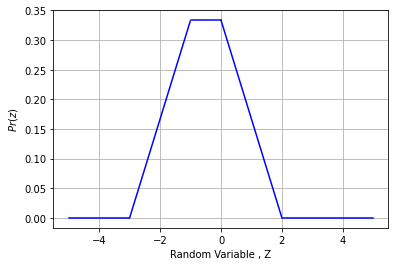
\includegraphics[width=.9\columnwidth] {solutions/ec/34/Figures/Assignment_3_PDF.png}
    \caption{The PDF of Z}
    \label{fig:The PDF of Z}
\end{figure}

\begin{figure}[!ht]
       \centering
    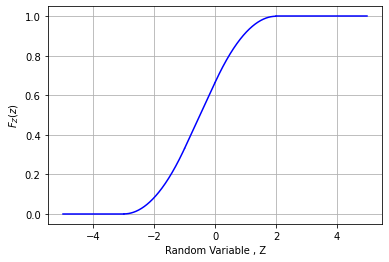
\includegraphics[width=.9\columnwidth] {solutions/ec/34/Figures/Assignment_3_CDF.png}
    \caption{The CDF of Z}
    \label{fig:The CDF of Z}
\end{figure}




%
\item Let $X_1$, $X_2$, $X_3$ and $X_4$ be independent normal random variables with zero mean and unit variance. The probability that $X_4$ is the smallest among the four is..... 
\\
\solution
Required probability
\begin{align}
    &= \pr{X_4 = min(X_1, X_2, X_3, X_4)}\\
    &= \int_{-\infty}^{\infty}\pr{X_1, X_2, X_3 > x | X_4 = x}
\end{align}
Since $X_1$, $X_2$, $X_3$ and $X_4$ are independent, required probability
\begin{align}
    &= \int_{-\infty}^{\infty} (1-F_{X_1}(x))(1-F_{X_2}(x))(1-F_{X_3}(x))f_{X_4}(x)dx\\
    &= \int_{-\infty}^{\infty} (1-\Phi(x))^3\phi(x)dx
\end{align}
Substituting 
\begin{align}
    u  &= 1 - \Phi(x)\\
    du &= -\phi(x)dx
\end{align}
we get required probability
\begin{align}
    = -\int_1^0 u^3 du\label{simplifiedintegral}\\
    = \cfrac{1}{4}
\end{align}
Note that in eq. \eqref{simplifiedintegral} the  integral is from 1 to 0 because
\begin{align}
    1-\Phi(-\infty) &= 1\\
    1-\Phi(\infty)  &= 0
\end{align}
Here $\phi(x)$ and $\Phi(x)$ represent the pdf and cdf of standard normal random variable respectively.

\item Let $A_{1},A_{2},.....A_{n}$ be n independent events in which the Probability of occurence of the event $A_{i}$ is given by P($A_{i}$) = 1 - $\frac{1}{\alpha^i}$, $\alpha >1$, i = 1,2,3,....n.Then the probability that atleast one of the events occurs is
\begin{enumerate}
    \item  1 - $\frac{1}{\alpha^\frac{n(n+1)}{2}}$ \hspace{0.95cm}
    \item  $\frac{1}{\alpha^\frac{n(n+1)}{2}}$\hspace{1.5cm}
    \\ \\
    \item  $\frac{1}{\alpha^n}$ \hspace{2.15cm}
    \item 1 - $\frac{1}{\alpha^n}$\hspace{0.95cm}
  \end{enumerate}
  %
  \solution
  Let $A_{1} + A_{2} + A_{3} .... + A_{n}$ = S, \\
$\pr{S}$ = Probability of atleast one event occuring
De morgan's law states that $(A + B)^\prime = A^\prime B^\prime$  
\begin{align}
    \label{1.1}
   \implies \pr{S} = 1 - \pr{S^\prime} \\ 
   %\label{1.2}
   1 - \pr{S^\prime}= 1 - \pr{A_{1}^\prime A_{2}^\prime A_{3}^\prime
   ....A_{n}^\prime}
   \label{ma2005:1}
\end{align}
$\forall$ i $\in$ {1,2,....n} \\
Since, $A_{i}$ are independent.\\
$\therefore$ Complements of $A_{i}$ are also independent.\\
$\implies$ 
\begin{equation}
%\label{2.1}
\pr{A_{1}^\prime A_{2}^\prime A_{3}^\prime
   ....A_{n}^\prime}=\prod_{i=1}^{n}\pr{A_{i}^\prime}
   \label{ma2005:2}
\end{equation}
\begin{equation}
%    \label{2.2}
\pr{A_{i}} = 1 - \frac{1}{\alpha^i} \implies \pr{A_{i}^\prime} = \frac{1}{\alpha^i} \label{ma2005:5}
\end{equation}
substituting \eqref{ma2005:5} in \eqref{ma2005:2},
\begin{equation}
    \label{2.3}
  \pr{A_{1}^\prime A_{2}^\prime A_{3}^\prime ....A_{n}^\prime} =  \prod_{i=1}^{n}\frac{1}{\alpha^i} \\
\end{equation}
\begin{equation}
\label{2.4}
   \prod_{i=1}^{n}\frac{1}{\alpha^i}=\frac{1}{\alpha^{\sum_{i}^{n}i}}= \frac{1}{\alpha^\frac{n(n+1)}{2}} 
\end{equation}
\begin{equation}
%\label{2.5}
    \therefore \pr{A_{1}^\prime A_{2}^\prime A_{3}^\prime ....A_{n}^\prime} = \pr{S^\prime} = \frac{1}{\alpha^\frac{n(n+1)}{2}} \label{ma2005:3}
\end{equation}
from equations \eqref{ma2005:1} and \eqref{ma2005:3} 
\begin{equation}
\label{2.6}
\implies \pr{S} = 1 - \pr{S^\prime} = 1 - \frac{1}{\alpha^\frac{n(n+1)}{2}}
\end{equation}
$\therefore$ The correct option is \textbf{(a)}
  %
  \item Let $X_{1},X_{2},\dots$, be a sequence of independent and identically distributed random variables with $P(X_{1}=1)=\dfrac{1}{4}$ and $P(X_{1}=2)=\dfrac{3}{4}$. If $\bar X_{n}=\dfrac{1}{n}\displaystyle\sum_{i=1}^{n}X_{i}$,  for $n=1,2,\dots$, then $\displaystyle\lim_{n\to\infty}P(\bar X_{n} \leq 1.8)$ is equal to
  \\
  \solution
  
Given,
\begin{align}
\tag{32.1}
    Pr(X_{1}=1)=\dfrac{1}{4},Pr(X_{2}=2)=\dfrac{3}{4}
\end{align}
As $X_{1},X_{2},\dots$, are identically distributed random variables, $\forall i \in \{1,2,\dots,n\}$
\begin{align}
\tag{32.2}
    Pr(X_{i}=1)=\dfrac{1}{4},Pr(X_{i}=2)=\dfrac{3}{4}
\end{align}
Also,
\begin{align}
\tag{32.3}
    \because P(X_{i}&=1)+P(X_{i}=2)=1\\
\tag{32.4}
    &\therefore X_{i} \in \{1,2\}
\end{align}
Therefore, each $X_{i}$ is a bernoulli distribution with
\begin{align}
\tag{32.5}
    p=\dfrac{3}{4},q=\dfrac{1}{4}
\end{align}
Let
\begin{align}
\tag{32.6}
    X=\displaystyle\sum_{i=1}^{n}X_{i}
\end{align}
be a binomial distribution. Its CDF is
\begin{align}
\tag{32.7}
    Pr(X\leq n+r)=\displaystyle\sum_{k=0}^{r}{\comb{n}{k}}p^{k}q^{n-k}
\end{align}
To find : $\displaystyle\lim_{n\to\infty}Pr(\bar X_{n} \leq a)$
\begin{align}
\tag{32.8}
    \bar X_{n} \leq a \Rightarrow X \leq na
\end{align}
Substituting $a(=1.8),p,q$, we get
\begin{align}
\tag{32.9}
    \displaystyle\lim_{n\to\infty}Pr(\bar X_{n} \leq 1.8)&=\displaystyle\lim_{n\to\infty}P(X\leq 1.8n)\\
\tag{32.10} 
    &=\displaystyle\sum_{k=0}^{0.8n}\dfrac{{\comb{n}{k}}3^{k}}{4^{n}}
\label{eq:val}
\end{align}
On solving \eqref{eq:val}, we get
\begin{align}
\tag{32.11}
    \displaystyle\lim_{n\to\infty}P(\bar X_{n} \leq 1.8)=1
\end{align}

  \item  Let $\{X_n\}_{n\ge 1}$ be a sequence of independent and identically distributed random variables each having uniform distribution on [0,3]. Let $Y$ be a random variable, independent of $\{X_n\}_{n\ge 1}$, having probability mass function
  \begin{align}
  \pr{Y=k} = 
  \begin{cases}
  \frac{1}{(e-1)k!} & k=1,2,3\cdots \\
  0 & otherwise
  \end{cases}
  \end{align}
  Then $\pr{max\{X_1,X_2,\cdots X_Y\}\le 1}$ equals ............\\
  %
  \solution
    
Given that $\{X_n\}_{n\ge 1}$ is having a uniform distribution on [0,3], so probability can be written as
\begin{align}
\pr{X_n}_{n\ge 1}=  
\begin{cases}
\frac{1}{3} & 0\le X_n\le 3 \\
0 & otherwise
\end{cases}
\end{align}
So,
\begin{align}
    \pr{X_n\le 1}_{n\ge 1}=\frac{1}{3}
\end{align}
Required probability
\begin{align}
 &=\pr{max\{X_1,X_2,\cdots X_Y\}\le 1}\label{st2021-48:req_prob}
 \end{align}
 Since, $\{X_n\}_{n\ge 1}$ is a sequence of independent variables and $Y$ is also independent of $\{X_n\}_{n\ge 1}$.\\
 And also in \eqref{st2021-48:req_prob}, the index of $X_i's$ depends on $Y$, so number of terms depends on $Y$, like if $Y=1$, then there is only $X_1$, if $Y=2$, then there's $X_1,X_2$, so required probability
\begin{align}
&=\sum_{p=1}^{\infty}\pr{max\{X_1,X_2,\cdots X_p\}\le 1|Y=p}\cdot \pr{Y=p}
\end{align}
\begin{align}
& =\sum_{p=1}^{\infty}\pr{max\{X_1,X_2,\cdots X_p\}\le 1}\cdot \pr{Y=p}\\
&=\sum_{p=1}^{\infty}\pr{X_1,X_2,\cdots X_p\le 1}\cdot \pr{Y=p}
\end{align}
\begin{multline}
=\sum_{p=1}^{\infty}\pr{X_1\le 1}\cdot \pr{X_2\le 1}\cdots \pr{X_{p-1}\le 1}\\
\cdot \pr{X_p\le 1}\cdot \pr{Y=p}
\end{multline}
\begin{align}
&=\sum_{p=1}^{\infty}\left(\frac{1}{3}\right)^p\left(\frac{1}{e-1}\right)\left(\frac{1}{p!}\right)\\
&=\left(\frac{1}{e-1}\right)\left[\sum_{p=0}^{\infty}\left(\frac{1}{3}\right)^p\left(\frac{1}{p!}\right)-1\right]
\label{st2021-48:taylor}
\end{align}
Using Taylor's Series of $e^x$ in \eqref{st2021-48:taylor}, \\
Required probability
\begin{align}
    &=\frac{e^{1/3}}{e-1}-\frac{1}{e-1}\\
    &=0.23
\end{align}
    

%
\item Let $X_1$, $X_2$ and $X_3$ be independent and identically distributed random variables with $E(X_1) = 0$ and $E\left(X^2_1\right)=\frac{15}{4}$. If $\psi : (0,\infty) \rightarrow (0,\infty)$ is defined through the conditional expectiation
$\psi(t) = E\left(X^2_1 | X_1^2 + X_2^2 + X_3^2 = t\right), t>0$
Then, $E(\psi((X_1+X_2)^2))$ is equal to,
%
\\
\solution
  It is given that $X_1$, $X_2$ and $X_3$ are independent and identically distributed random variables.
\begin{align}
    \nonumber E\left(X^2_1 | X_1^2 + X_2^2 + X_3^2 = t\right) &= 
    E\left(X^2_2 | X_1^2 + X_2^2 + X_3^2 = t\right)\\ &= 
    E\left(X^2_3 | X_1^2 + X_2^2 + X_3^2 = t\right)\label{ma2015-28:eq:2.0.1}
\end{align}
Now,
\begin{align}
   \nonumber &\sum_{n=1}^3 E\left(X^2_n | X_1^2 + X_2^2 + X_3^2 = t\right)\\ &= E\left(X_1^2 + X_2^2 + X_3^2 | X_1^2 + X_2^2 + X_3^2 = t\right)\\
   &= t
\end{align}
Hence, from \eqref{ma2015-28:eq:2.0.1}.
\begin{align}
     E\left(X^2_1 | X_1^2 + X_2^2 + X_3^2 = t\right) &= \frac{t}{3}\\
     \therefore \psi(t) &= \frac{t}{3}\label{ma2015-28:eq:2.0.5}
\end{align}
Hence, from \eqref{ma2015-28:eq:2.0.5},
\begin{align}
    E(\psi((X_1+X_2)^2)) &= E\left(\frac{(X_1+X_2)^2)}{3}\right)\\
    &= E\left(\frac{X_1^2 + X_2^2 + 2X_1\times X_2}{3}\right)\\
    &= \frac{E(X_1^2) + E(X_2^2) + 2\times E(X_1) \times E(X_2)}{3}\\
    &= \frac{\frac{15}{4}+\frac{15}{4}+ 2\times0\times0}{3}\\
    &= \frac{15}{6}\\
    \therefore E(\psi((X_1+X_2)^2)) &= 2.5
\end{align}

%
\item Let $X \sim B\brak{5,\frac{1}{2}}$ and $Y \sim U(0,1)$. The the value of:
\[
    \frac{\pr{X+Y \leq 2}}{\pr{X+Y \geq 5}}
\]
is equal to? ($X$ and $Y$ are independent)
\solution 
  Characteristic function for $X \sim B\brak{5,\frac{1}{2}}$ will be:
\begin{align}
    C_X(t)=\brak{\frac{e^{it}+1}{2}}^5
\end{align}
Characteristic function for $Y \sim U(0,1)$ will be:
\begin{align}
    C_Y(t)=\frac{e^{it}-1}{it}
\end{align}
Since both $X$ and $Y$ are independent we can take:
\begin{align}
    Z&=X+Y\\
    C_Z(t)&=C_X(t)C_Y(t)\\
    C_Z(t)&= \frac{(e^{it}+1)^5(e^{it}-1)}{32it}
\end{align}
Applying Gil-Pelaez formula:
\begin{align}
    F_Z(z)=\frac{1}{2}-\frac{1}{\pi}\int_0^\infty \frac{\text{Im}\brak{e^{-itz}C_Z(t)}}{t}dt
\end{align}
\begin{multline*}
    F_Z(z)=\frac{1}{2}-\frac{1}{\pi}\int_0^\infty\frac{1}{2it}\brak{\frac{(e^{it}+1)^5(e^{it}-1)e^{-itz}}{32it}}\\+\frac{1}{2it}\brak{\frac{(e^{-it}+1)^5(e^{-it}-1)e^{itz}}{32it}}dt
\end{multline*}
Substituting $z=2$, the value for $\pr{Z\leq 2}$:
\begin{align}
\nonumber
    &=\frac{1}{2}+\frac{1}{\pi}\int_0^\infty \frac{8\cos{2t}+2\cos{4t}}{64t^2}dt\\
    &\quad+\frac{1}{\pi}\int_0^\infty\frac{+8\cos{3t}-8\cos{t}-10}{64t^2}dt\label{challenge/1first_sub}
\end{align}
Finding a general expression for integrating:
\begin{align}
    \int \frac{\cos{ax}}{x^2}dx=-\frac{\cos{ax}}{x}-a\int\frac{\sin{ax}}{x}dx + C\label{challenge/1gen1}
\end{align}
By applying integration by parts. Now finding the value of other integral, by substituting $u=ax$ for limits as $0$ and $\infty$:
\begin{align}
    \int_0^\infty\frac{a\sin{ax}}{x}dx &= \int_0^\infty\frac{a\sin{u}}{u}du\\
    &=\frac{a\pi}{2}\label{challenge/1gen2}
\end{align}
Now using the above general expressions to calculate \eqref{challenge/1first_sub} and simplifying the expression after putting the limits we get
\begin{align}
    &=\frac{-1}{8\pi}\brak{\int_0^\infty\frac{\sin{4t}+3\sin{3t}+2\sin{2t}-\sin{t}}{t}dt}\\
    &\quad -\frac{2(\cos{t}-1)(\cos{t}+1)^3}{8\pi t}\bigg|_0^\infty+\frac{1}{2}\\
    &=\frac{1}{2} + \frac{-1}{8\pi}\times \frac{5\pi}{2}+0\\
    &=\frac{3}{16}\label{challenge/1first_value}
\end{align}
Using \eqref{challenge/1gen2} and \eqref{challenge/1gen1} to calculate for our second case
Similarly on substituting $z=5$, the value for $\pr{Z\leq 5}$:
\begin{align}
\nonumber
    &=\frac{1}{2} +\frac{1}{\pi}\int_0^\infty\frac{-10\cos{3t}-8\cos{4t}}{64t^2}dt\\&\quad +\frac{1}{\pi}\int_0^\infty\frac{-2\cos{5t}+12\cos{t}+8}{64t^2}dt\\ \nonumber
    &=\frac{1}{\pi}\brak{\int_0^\infty\frac{5\sin{5t}+16\sin{4t}+15\sin{3t}-6\sin{t}}{32}dt}\\
    &\quad+\frac{1}{2}+\frac{1}{\pi}\brak{\frac{16(\cos{t}-1)(\cos{t})(\cos{t}+1)^3}{32t}\bigg|_0^\infty}\\
    &=\frac{1}{2}+\frac{1}{\pi}\times\frac{15\pi}{32} + 0\\
    &=\frac{31}{32}
\end{align}
The value for $\pr{Z\geq 5}$:
\begin{align}
    \pr{Z>5}&=1-\pr{Z\leq 5}\\
    &=1-\frac{31}{32}=\frac{1}{32}\label{challenge/1second_value}
\end{align}
Upon substituting \eqref{challenge/1first_value}and \eqref{challenge/1second_value}, we get:
\begin{align}
    \frac{\pr{X+Y \leq 2}}{\pr{X+Y \geq 5}} = 6
\end{align}

\item A die is thrown again and again until three sixes are obtained.Find the probability of obtaining the third six in the sixth row of a die.
\end{enumerate}